\documentclass[thesis.tex]{subfiles}

\begin{document}
\ifSubfilesClassLoaded{
    \setcounter{chapter}{7}
}

\chapter{Estimating transmission using mechanistic modelling} \label{SEIR}

This chapter uses mechanistic models for estimating the transmission of SARS-CoV-2.
This is an alternative approach to the statistical methods used in \cref{E-backcalc}.
Mechanistic models explicitly represent the infection process driving the spread of infectious disease.
The explicit representation means that a mechanistic model's state and parameters have biological and/or epidemiological interpretations; these interpretations provide scientific understanding of the disease.
Of particular interest is that the basic reproduction number, $R_0$, and the effective reproduction number, $R_e(t)$, can both be calculated as simple functions of the model parameters; using \cref{E-backcalc} additional modelling would be required to estimate these numbers.
Furthermore, mechanistic models can be used for scenario-based modelling, whereby the effect of different interventions can be simulated.
All of these properties make mechanistic models a useful tool for understanding and controlling infectious diseases.
However, they make stronger assumptions about the disease than statistical models, and often perform worse in short-term forecasting\todo{add a citation}.

\Cref{SEIR:sec:transmission-generic} introduces a generic framework for mechanistic modelling of infectious diseases.
% This framework is then applied to SARS-CoV-2 in \cref{SEIR:sec:transmission-application}.
It describes the \emph{transmission model}, corresponding to the infection process (see \cref{E-inc-prev:sec:infection-process}).
The transmission model needs to be linked to observations; in this chapter, that will be the CIS prevalence data.
The \emph{observation model}, introduced in \cref{SEIR:sec:observation}, is this link; it incorporates both the prevalence process (see \cref{E-inc-prev:sec:prevalence-process}) and the observation process (see \cref{E-inc-prev:sec:observation-process}).
\Cref{SEIR:sec:inference-implementation} describes the inference process, parameterisation, and priors for this model.
I ensure that the model can recover the parameters successfully in a simulation study in \cref{SEIR:sec:sim-study} before applying it to the CIS data in \cref{SEIR:sec:application}, which includes comparisons to the results in \cref{E-backcalc}.
Finally, \cref{SEIR:sec:discussion} discusses the results, limitations, and extensions of this work.

The literature on mechanistic models is vast, having been developed for over a century; the model in \cref{SEIR:sec:SIR} was first formulated in the 1920s~\autocite{kermackContribution}.
This chapter explains only the background I will use in the application to SARS-CoV-2.
For further details I recommend the tutorial paper \textcite{kretzschmarMathematical} or the textbook \textcite{keelingModeling}.

Notation in this chapter differs from the rest of this thesis.
I adopt conventions and notation from the infectious disease modelling field, although this is not consistent in the literature.
In particular, case no longer signifies whether a variable is random or not, but will be clear from the context.

\section{Transmission models} \label{SEIR:sec:transmission-generic}

\todo[inline]{ref intro to compartmental model setup}
This section introduces the class of mechanistic transmission models known as \emph{compartmental} models.
Compartmental models are the most widely-used class of mechanistic infectious disease model.
A compartmental model is named because they place every member of the population under study into a compartment; each compartment represents a disease state (\eg susceptible).

A compartmental model consists of a state vector $\vec{x}(t)$ and a set of parameters $\vec{\theta}$.
The elements of $\vec{x}(t)$ are the proportion of the population (or number of individuals) in each compartment at time $t$.
The parameters $\vec{\theta}$ are constants that determine, along with the model structure, how the state vector changes over time.
Compartmental models can be \emph{deterministic} or \emph{stochastic}.
Deterministic models are defined by the state vector $\vec{x}(t)$ being a deterministic, although rarely analytically-tractable, function of the parameters $\vec{\theta}$ and the initial state $\vec{x}(0)$.
%The transmission model corresponds to the infection process (see \cref{E-inc-prev:sec:infection-process}).
%There remains randomness in the observation model (described in \cref{SEIR:sec:observation}).
Stochastic models are most commonly specified in discrete time, using a Markov assumption.
That is, they specify a probability distribution $p(\vec{x}(t) \mid \vec{x}(t-1), \vec{\theta})$.
This relaxes the assumption of independent increments in the counting process formulation of the infection process (see \cref{E-inc-prev:sec:infection-process}).

Deterministic models are also known as \emph{mean-field} models because they can are the behaviour corresponding to a stochastic model's mean.
When the number of infected individuals is large, the law of large numbers means that the mean-field behaviour is a good approximation of the fully stochastic model~\autocite[20]{diekmannMathematical}.
An alternative justification, when making noisy observations of the system, is that the additional noise from the stochastic model is negligible compared to this observation noise.
This second justification is of the same form as the one made for neglecting the stochasticity of the prevalence process in \cref{E-inc-prev:sec:observation-process}.
The remainder of this chapter uses only deterministic models, because throughout the time period this thesis considers there were enough infectious individuals.
For an introduction to stochastic models, see \textcite[chapter 6]{keelingModeling}.
% \todo{Maybe say something about still having a stochastic observation model, if not clear enough from intro}

In particular, this chapter discusses deterministic models whose evolution is specified by a system of ODEs, $d\vec{x}/dt$.
Therefore, in an ODE model, time is necessarily continuous, although discretised when solving (see \cref{SEIR:sec:inference-implementation}).
For concreteness, I use units of days throughout, although the model can use any unit of time.
The number or proportion of individuals in each compartment is also continuous, which is a reasonable approximation when the population is large.

\Cref{SEIR:sec:SIR} introduces the \emph{susceptible-infected-recovered} (SIR) model, a simple compartmental model for a disease which confers immunity.
The SIR model is named because each individual in the population is divided into one of three states: susceptible, infectious, or recovered.
This model has several assumptions which make it inappropriate to model SARS-CoV-2; therefore, the remainder of this sections relaxes these assumptions.
First, \cref{SEIR:sec:non-exponential} relaxes the assumption of an exponentially-distributed infectious period to a gamma distribution.
Then, \cref{SEIR:sec:SEIR} relaxes the assumption that individuals are infectious immediately after they are infected; it does this by extending the SIR model to the SEIR model, including an \emph{exposed} compartment.
Finally, \cref{SEIR:sec:structured-populations} allows heterogeneity in the population, introducing stratification by important characteristic(s).
% Finally, \cref{SEIR:sec:time-varying-foi} relaxes the assumption of a constant transmission rate to allow for time-varying behavioural changes.


\subsection{The SIR model} \label{SEIR:sec:SIR}

\begin{figure}[h]
\makebox[\textwidth][c]{
\begin{tikzpicture}[
    node distance = 2.5cm,
    on grid,
    auto,
    ->,>=stealth',
    every state/.style={draw,rectangle},
    ]

    \node[state] (S) {$s$};
    \node[state, right=of S] (I) {$i$};
    \node[state, right=of I] (R) {$r$};

    \path (S) edge node {$\lambda(t)$} (I)
          (I) edge node {$\gamma$} (R);
\end{tikzpicture}
}
  \caption[The SIR model]{Schematic of the basic SIR model. Arrows are labelled with the rates at which individuals move between compartments.}
  \label{SEIR:fig:SIR}
\end{figure}

The simplest compartmental model for a disease which confers immunity is the (SIR) model\todo{ref for SIR being simplest}.
The name refers to the three compartments in the model, displayed in \cref{SEIR:fig:SIR}.
Individuals in the susceptible compartment are those that could be infected (they have no immunity).
The proportion of the population that is susceptible at time $t$ is $s(t)$.
Individuals in the infectious compartment can infect others, and eventually recover.
The proportion of the population that is infectious at time $t$ is $i(t)$.
Individuals in the recovered compartment are immune to the disease, and cannot be infected again.
The proportion of the population that have recovered by time $t$ is $r(t)$.
The model's state is $\vec{x}(t) = (s(t), i(t), r(t))^T$.
In the SIR model, individuals are assumed to be homogeneous, \ie they are all identical.

The SIR model is described by the following system of ODEs~\autocite[19]{keelingModeling}:
\begin{align}
\frac{ds(t)}{dt} &= -\lambda(t) s(t) \\
\frac{di(t)}{dt} &= \lambda(t) s(t) - \gamma i(t) \\
\frac{dr(t)}{dt} &= \gamma i(t)
\end{align}
where $\lambda(t) = \beta i(t)$, is the \emph{force of infection}: the risk of infection for a susceptible individual at time $t$~\autocite[17]{keelingModeling}.
Two parameters are present in this model: $\beta$ and $\gamma$, \ie $\vec{\theta} = (\beta, \gamma)^T$.
$\beta$ is the transmission rate, absorbing several terms as described below.
%\todo{check what beta is called: effective transmission rate or transmission rate or something else?}, or the number of individuals an infected individual infects per day.
$\gamma$ is the recovery rate, or the proportion of infected individuals that recover per day; hence, $1/\gamma$ is the mean infectious period~\autocite[367]{keelingModeling}.
These parameters are assumed to be constant.

% The term $\beta s(t)i(t)$ is the rate at which susceptible individuals (as a proportion of the total population size) are infected~\autocite[18]{keelingModeling}.
% Susceptible individuals move from the $s(t)$ to $i(t)$ when they are infected.
The expression for the force of infection, $\lambda(t)$ can be arrived at by considering a single infected individual~\autocite[214]{kretzschmarMathematical}.
Assume this individual, on average, comes into contact with other individuals in the population at a rate of $\kappa$ per day.
Further, assume the population is \emph{well-mixed}, meaning that each contact is with an individual chosen uniformly at random from the population; this is implied by assuming a homogeneous population.
For such a randomly selected individual, the probability that they are susceptible is $s(t)$.
% Each of the infected individual's contacts is therefore with a susceptible individual with probability $s(t)$, by the well-mixed assumption.
Therefore, in expectation, the infected individual makes contact with susceptible individuals at a rate of $\kappa s(t)$.
Assume that there is a constant probability of transmission upon contact between an infected and susceptible individual, $q$.
Combined with the above, the expected rate of infections caused by this infected individual is $\kappa s(t) q$.
The two constant terms here (number of contacts and probability of transmission) are absorbed into the transmission rate, $\beta = \kappa q$.
Therefore, the rate of new infections generated by a single infectious individual is $\beta s(t)$.
Multiplying by the number of infected individuals and dividing by the population size gives the rate at which susceptible individuals are infected as a proportion of the population, $\beta s(t) i(t) = \lambda(t) s(t)$.

% The term $\gamma i(t)$, the rate at which infected individuals (as a proportion of the total population size) recover, follows directly from the definitions of $\gamma$ and $i(t)$.

A few properties and assumptions of the SIR model are worth noting.
\begin{itemize}
    \item The basic reproduction number for this model is $R_0 = \beta / \gamma$~\autocite[20]{keelingModeling}.
    Intuitively, this can be thought of as the average number of infections caused by an infectious individual per day, $\beta$, multiplied by the average number of days they are infectious for, $1/\gamma$.
    \item The effectie reproduction number for this model is $R_e(t) = \beta / \gamma s(t) = R_0 s(t)$~\autocite{pellisEstimation}.
    \item The population is closed.
    That is, the total population size is constant, and no infections are imported from outside the population.
    Births and deaths of individuals are also excluded, although they can easily be incorporated in situations where they are relevant~\autocites[26]{keelingModeling}[214]{kretzschmarMathematical}.
    \item There is no analytical solution to the system of ODEs: numerical methods are required to solve the system~\autocite[25]{keelingModeling}.
    \item In addition to the parameters, the state of the system at some time (normally the initial state, the state at time $t=0$) is required to solve the system.
    \item Immunity is assumed to last until the end of the modelled period~\autocite[61]{andersonInfectious}.
    In many contexts, including here, this assumption is justified because the modelled period is shorter than the length of immunity conferred~\autocite{milneImmunity}.
    For modelling longer time periods, waning immunity can be incorporated by allowing individuals to move from the recovered compartment back to the susceptible compartment~\autocite[40]{keelingModeling}.
\end{itemize}


\subsection{Non-exponential waiting times} \label{SEIR:sec:non-exponential}
\begin{figure}[h]
\makebox[\textwidth][c]{
\begin{tikzpicture}[
    node distance = 2.5cm,
    on grid,
    auto,
    ->,>=stealth',
    every state/.style={draw,rectangle},
    ]

    \node[state] (S) {$s$};
    \node[state, right=of S] (I1) {$i_1$};
    \node[state, right=of I1] (I2) {$i_2$};
    \node[state, right=of I2, draw=none] (I3) {$\cdots$};
    \node[state, right=of I3] (I4) {$i_n$};
    \node[state, right=of I4] (R) {$r$};

    \path (S) edge node {$\beta i$} (I1)
          (I1) edge node {$n\gamma$} (I2)
          (I2) edge node {$n\gamma$} (I3)
          (I3) edge node {$n\gamma$} (I4)
          (I4) edge node {$n\gamma$} (R);
\end{tikzpicture}
}
  \caption[The SIR model with non-exponential infectious period]{Schematic of the SIR model with non-exponential infectious period. The infectious period is modified by having multiple I states.}
  \label{SEIR:fig:SIR-gamma}
\end{figure}

The basic SIR model implies that the distribution of the time spent in the infected compartment is exponential~\autocite[96]{keelingModeling}.
This is an unrealistic assumption for most diseases and leads to an underestimation of the reproduction number if the model is fit to data~\autocites{lloydRealistic}{wearingAppropriate}.
A standard extension to the SIR model is to allow the infectious period to follow a gamma distribution~\autocite[94]{keelingModeling}.
This is done by adding multiple infected compartments (see \cref{SEIR:fig:SIR-gamma}).
The system can now be written as follows:
\begin{align}
\frac{ds(t)}{dt} &= -\lambda(t) s(t)\\
\frac{di_1(t)}{dt} &= \lambda(t) s(t) - n\gamma i_1(t) \\
\frac{di_2(t)}{dt} &= n\gamma i_1(t) - n \gamma i_2(t) \\
&\vdots \nonumber \\
\frac{di_n(t)}{dt} &= n\gamma i_{n-1}(t) - n \gamma i_n(t) \\
\frac{dr(t)}{dt} &= n\gamma i_n(t)
\end{align}
where $n$ is the number of infected compartments, and redefining $\lambda(t) = \beta \sum_{j=1}^n i_j(t)$.
In this model the infectious period is distributed $\GamDist(n, n\gamma)$, a realistic model for a variety of diseases~\autocite{wearingAppropriate}.
This parameterisation is chosen to give $1/\gamma$ as the mean infectious period (the gamma distribution's definition and its expectation are in \cref{E-distributions}).
% (it is slightly unclear what it means for a variable to have a distribution in a deterministic model, the clearest explanation is that this is the distribution which the ).
A gamma distribution with the first parameter equal to 1 is an exponential distribution, in which case this model collapses to the basic SIR model in \cref{SEIR:sec:SIR}.
The distribution for the time spent in the infected compartments tends to a constant (\ie the same for all individuals) as $n \to \infty$~\autocite{lloydRealistic}.
The reproduction number in terms of the parameters is unchanged by this extension, \ie $R_0 = \beta / \gamma$.

\subsection{The SEIR model} \label{SEIR:sec:SEIR}

\begin{figure}[h]
\makebox[\textwidth][c]{
\begin{tikzpicture}[
    node distance = 2cm,
    on grid,
    auto,
    ->,>=stealth',
    every state/.style={draw,rectangle},
    % remember picture, overlay
    ]

    \node[state, xshift=-2cm] (S) {$s$};
    \node[state, right=of S] (E1) {$e_1$};
    \node[state, right=of E1] (E2) {$e_2$};
    \node[state, right=of E2, draw=none] (E3) {$\cdots$};
    \node[state, right=of E3] (E4) {$e_m$};
    % \node[state, right=of E4] (I1) {$i_1$};
    \node[state, below=of E1] (I1) {$i_1$};
    \node[state, right=of I1] (I2) {$i_2$};
    \node[state, right=of I2, draw=none] (I3) {$\cdots$};
    \node[state, right=of I3] (I4) {$i_n$};
    \node[state, right=of I4] (R) {$r$};

    \path (S) edge node {$\beta i$} (E1)
          (E1) edge node {$m\sigma$} (E2)
          (E2) edge node {$m\sigma$} (E3)
          (E3) edge node {$m\sigma$} (E4)
          (I1) edge node {$n\gamma$} (I2)
          (I2) edge node {$n\gamma$} (I3)
          (I3) edge node {$n\gamma$} (I4)
          (I4) edge node {$n\gamma$} (R);
    \draw[->] (E4.east) -- ++(1,0) |- ([yshift=-1cm]E4.east) node [near start, right] {$m\sigma$} -|  (I1.north);
\end{tikzpicture}
}
  \caption[The SEIR model]{Schematic of the SEIR model.}
  \label{SEIR:fig:SEIR}
\end{figure}

The SIR model assumes that individuals are immediately infectious upon infection.
This is unrealistic for most diseases, as there is a period between an individual being infected and them being infectious, known as the \emph{latent period}.
\todo{I will probably end up defining the latent period in the intro, so should just ref that}
Ignoring the latent period will again overestimate the reproduction number~\autocite{wearingAppropriate}.

The SIR model can be extended to include a latent period by adding a latent compartment~\autocite[41]{keelingModeling}.
This is also known as an \emph{exposed} compartment.
Therefore, we now form the susceptible-exposed-infected-recovered (SEIR) model, shown in \cref{SEIR:fig:SEIR}.

Similar to the exponential infectious period, the latent period can be modelled as a gamma distribution by adding multiple latent compartments.
\begin{align}
\frac{ds}{dt} &= -\beta si \\
\frac{de_1}{dt} &= \beta si - m\sigma e_1 \\
\frac{de_2}{dt} &= m\sigma e_1 - m \sigma e_2 \\
&\vdots \nonumber \\
\frac{de_m}{dt} &= m\sigma e_{m-1} - m \sigma e_m \\
\frac{di_1}{dt} &= m\sigma e_m - n\gamma i_1 \\
\frac{di_2}{dt} &= n\gamma i_1 - n \gamma i_2 \\
&\vdots \nonumber \\
\frac{di_n}{dt} &= n\gamma i_{n-1} - n \gamma i_n \\
\frac{dr}{dt} &= n\gamma i_n
\end{align}
where $m$ is the number of latent compartments and $1/\sigma$ is the mean latent period.
The latent period is distributed $\GamDist(m, m\sigma)$.
The infectious period is still distributed $\GamDist(n, n\gamma)$.

The reproduction number in terms of the parameters is unchanged by this extension, \ie $R_0 = \beta / \gamma$, however, the growth rate in the exponential phase will be slower than before~\autocite[41]{keelingModeling}.

\subsection{Structured populations} \label{SEIR:sec:structured-populations}

To relax the assumption of a homogeneous population, the population can be stratified.
If the strata have differing transmission patterns, this can change the dynamics of the epidemic.
The different patterns could be due to behavioural factors (\eg high-numbers of sexual partners in a sexually-transmitted disease~\autocite[69]{keelingModeling}, younger age groups making many more contacts for respiratory diseases~\autocite[176]{andersonInfectious}), or biological factors (\eg genetics reducing the susceptibility of some individuals~\autocite[208]{andersonInfectious}).
I will assume that the disease progression (\eg length of the exposed and infectious periods) is the same for all strata, although this assumption can be relaxed.
Stratification requires two major changes model changes: extension of the state vector and describing the between-strata interactions.

The state vector is now a vector of vectors, one for each of the compartments.
I denote the set of strata, as $\set{A}$, with the set's size as $A$.
For example, in the basic SIR model, $\vec{x}(t) = (\vec{s}(t), \vec{i}(t), \vec{r}(t))^T$.
The $a$th element of each vector is the proportion of strata $a$ in that compartment.
For example, $\vec{s}(t) = (s_1(t), \dots, s_A(t))^T$ where $s_a(t)$ is the proportion of the $a$th strata that are susceptible at time $t$.
Hence, $N_a s_a(t)$ is the number of susceptible people in stratum $a$.
These vectors simply replace the scalars in the previous equations.
Various other definitions are possible and equivalent, for example defining $s_a$ as the proportion of the total population that are both in strata $a$ and susceptible or parameterised using numbers of individuals~\autocite[57]{keelingModeling}.

The interactions between strata also need describing.
This is done by replacing the scalar $\beta$ with a \emph{Who Acquires Infection From Whom} (WAIFW) matrix, $\matr{\beta}$~\autocite[58]{keelingModeling}; its interpretation is described below.
The force of infection is now a vector, $\vec\lambda(t) = \matr{\beta} \sum_{j=1}^n \vec{i_j}(t)$.
Its expression can be arrived at by considering a single infected individual in strata $a'$.
Assume any such individual comes into contact with individuals in strata $a$ at a rate of $\kappa_{aa'}$ in units of contacts per day.
% Further, assume that each contact is with an individual chosen uniformly at random from within the strata.
% For such a randomly selected individual, the probability that they are susceptible is $s_a(t)$.
% Each of the infected individual's contacts is therefore with a susceptible individual with probability $s(t)$, by the well-mixed assumption.
Following the same argument as in \cref{SEIR:sec:SIR} finds that, in expectation, the infected individual makes contact with susceptible individuals in stratum $a$ at a rate of $\kappa_{aa'} s_a(t)$.
Assume that there is a constant probability of transmission upon contact between an infected in strata $a'$ and susceptible in strata $a$ individual, $q_{aa'}$.
Therefore, the expected rate of infections in strata $a$ caused by this infected individual is $\kappa_{aa'} s_a(t) q_{aa'}$.
Multiplying by the number of infected individuals in strata $a'$, $N_{a'} i_{a'}(t)$, gives $\kappa_{aa'} q_{aa'} s_a(t) N_{a'} i_{a'}(t)$.
The constant terms here are absorbed into the WAIFW matrix, giving $\beta_{aa'} = \kappa_{aa'} q_{aa'} N_{a'}$.
The total force of infection on strata $a$ from all strata is, therefore, $\lambda_a(t) = \sum_{a' \in \set{A}} \beta_{aa'} i_{a'}(t)$.
Equivalently, $\vec\lambda(t) = \matr{\beta} \sum_{j=1}^n \vec{i_j}(t)$.
If all $\beta_{aa'}$ are equal, then the model is equivalent to the homogeneous model (\ie without any structure).
The rate that individuals move between the susceptible and exposed compartments is now $\vec{s}(t) \circ \vec\lambda(t)$, where $\circ$ denotes element-wise multiplication.

In practical situations, estimating all of the $\beta_{aa'}$ parameters is infeasible, so some assumptions must be made to reduce the number of parameters~\autocite[176]{andersonInfectious}.
The infeasibility arises because the progression of the epidemic depends on $\vec{\lambda}(t)$, which has dimension $A$, while $\matr{\beta}$ has dimension $A^2$.
Common assumption include assuming symmetry, \ie $\beta_{aa'} = \beta_{a'a}$, or that the direction of transmission is irrelevant, \ie $\beta_{aa'} = \beta_{a} \beta_{a'}$.
Alternatively, as in the scalar case, $\beta_{aa'}$ can be decomposed into the contact rate between strata $a$ and $a'$, $\kappa_{aa'}$ and the probability of transmission upon contact, $q_{aa'}$, and then assumptions made about the components.
The choice of assumptions depends on the context, including the disease being studied and the data available.

Reproduction numbers in models with structured populations need to be careful to consider the distribution of infections across the strata.
The WAIFM allows calculation of the number of secondary infections generated by a single infection in the $a$th strata.
This follows directly from its definition as $\frac{1}{\gamma} \sum_{a'} \beta_{aa'}$. 
However, how to average these contributions to form the reproduction is not obvious.
The standard solution to this was proposed by \textcite{diekmannDefinition} (although \textcite[chapter 7]{diekmannMathematical} provides a more gentle, but still rigorous, explanation).
First, they show that the distribution of infections across the strata during the initial period of exponential growth (when $\vec{s} \approx \vec{0}$) relies only on $\matr{\beta}$.
The distribution is proportional to the \emph{dominant eigenvector} (the eigenvector corresponding to the largest eigenvalue) of $\matr{\beta}$.
Denote by $\rho(\matr{\beta})$ the \emph{dominant eigenvalue} (the largest eigenvalue).
The basic reproduction number is then defined as $R_0 = \rho(\matr{\beta}) / \gamma$.
This $R_0$ keeps the same interpretation as in the homogeneous case, \ie the average number of secondary infections caused by a single infection in a fully susceptible population, where the average is taken over the distribution implied by the dominant eigenvector.
The important threshold that exponential growth occurs (in expectation) iff $R_0 > 1$ remains.

Based primarily on the study of influenza, age-based contact patterns have been found to be important for respiratory diseases~\autocites{birrellRealtimea}{jacksonEffects}.
\todo{maybe better ref for influence of age contacts on respiratory diseases}
Respiratory diseases can be spread by conversational contacts, which show very clear age patterns (see \cref{SEIR:fig:age-contacts}).
In particular, the contacts are \emph{associative} (contacts are more likely between individuals of similar ages) and younger age groups have more contacts; this will tend to concentrate the epidemic in these younger age groups~\autocite[67]{keelingModeling}.
\begin{figure}
  \centering 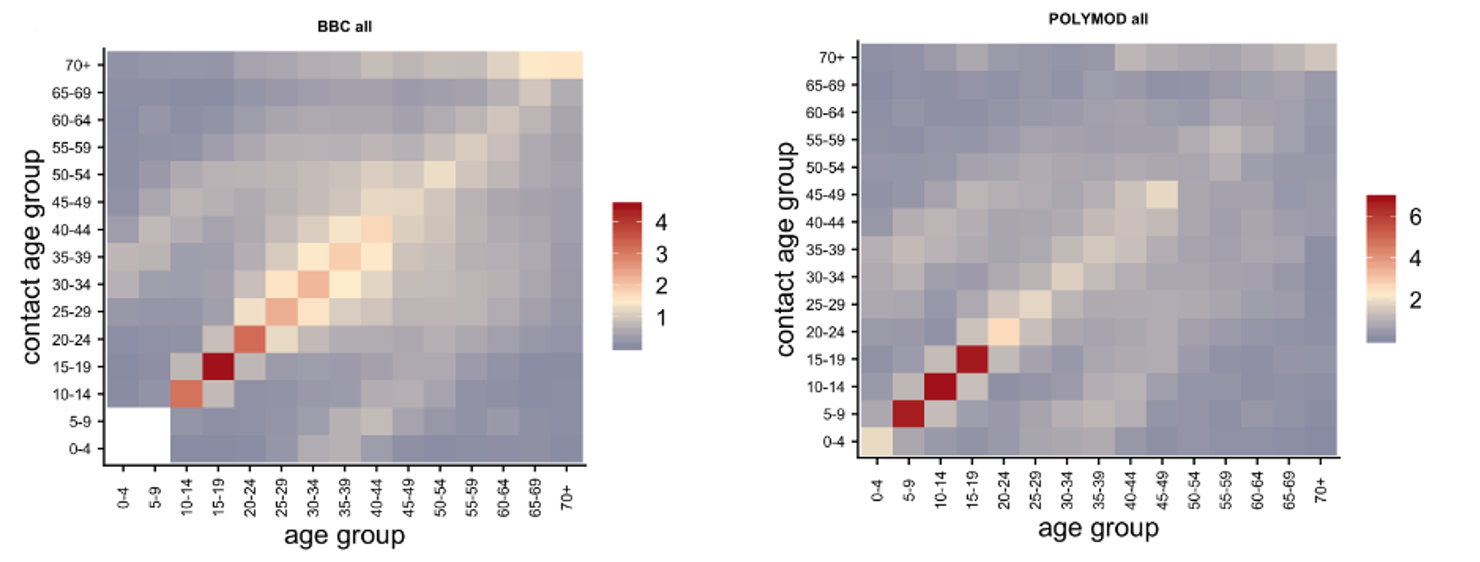
\includegraphics[width=\textwidth]{SEIR/contact_matrices}
  \caption[Age-based contact matrices]{Number of contacts reported between age groups in two contact surveys. Left shows the number of contacts reported in the POLYMOD survey~\autocite{mossongSocial}. Right shows the number of contacts reported in the BBC Pandemic survey~\autocite{klepacContacts}, which only collected data on those aged over 12. A clear diagonal, showing associative mixing is visible, and children have more contacts. Parallel diagonals off the main diagonal show mixing between parents and their children. Figure adapted from \textcite{klepacContacts}.}
  \label{SEIR:fig:age-contacts}
\end{figure}


% \section{A transmission model for SARS-Cov-2} \label{SEIR:sec:transmission-specific}

% I follow \textcite{birrellRealtimea} in parameterising $\matr{\beta}$, which includes introducing a time-dependency.


\section{Observation model} \label{SEIR:sec:observation}
\todo[inline]{Be clear this section is to fit to CIS data}

A variety of different approaches can be taken to link a transmission model to observations.
% Here, I extend the system of ODEs to include compartments representing PCR positive individuals.
% The proportion of PCR positive individuals in each strata is then linked to the CIS using a Beta-Binomial likelihood, with the modelled proportion that are PCR positive as the mean of the Beta distribution.
One approach would be to convolve the incidence based on the transmission model with the PCR duration distribution.
\todo{tidy up this notation}
Essentially, using the notation of \cref{E-inc-prev}, calculate the expected proportion of positive tests on day $t$ as $P_t = \sum_{j=1}^{\dmax} Z_{t-j} S(j)$.
$Z_{t-j}$ can be related to the ODEs because $Z_t / \Npop = s(t) - s(t-1)$, as $s(t)$.
However, this approach is computationally expensive.

A much more efficient option is to approximate this convolution by adding compartments to the ODEs.
This approach also allows the infected, pre-positive compartment to be represented.
I will denote this new compartment as $p_0$.
$p_0$ increases at the same rate as individuals flow into $e_1$.
These individuals then transition into a set of compartment with their transition rates chosen to match the duration of positivity estimates in \cref{E-imperf-test}, $p_1, \dots, p_l$.
These compartments do not have a biological interpretation, unlike the other compartments in the system, but are purely a mathematical tool so that the time spent in these compartments matches the duration distribution.
This is the same idea behind having multiple exposed or latent compartments (introduced in \cref{SEIR:sec:non-exponential}).

The class of distributions which can be represented as a series of compartments are known as \emph{phase-type} distributions.
Discussions of general phase-type distributions are beyond the scope of this thesis; a review in a biological context can be found in \textcite{hobolthPhasetype}.
I will restrict myself to the subset of phase-type distributions defined by \textcite{osogamiClosed} as Erlang-Coxian (EC) distributions.
EC distributions are convenient because they are flexible enough to approximate almost any distribution, and the parameters of the approximation are given by closed-form functions of the distribution's moments.

% Formally, a phase-type distribution as the distribution of \emph{absorption time} in a \emph{continuous-time Markov process} with a single absorbing state~\autocite{hobolthPhasetype}.
% Given a probability distribution over starting states, a rate at which 
% The process can be defined by its size, $l$, a $l \times l$ \emph{transition matrix}, $\matr{M} \in \reals^{l \times l}$, an \emph{exit rate} vector, $\vec{\alpha}$ 
% The process's state at time $t$, $W_t$, is a scalar $W_t \in \{ 1, \dots, l+1 \}$.
% Its transition matrix is defined, for $j \neq k$, as $\prob(W_{t+\delta t} = k \mid ) = M_{jk} \delta t$ for small, positive $\delta t$.
% The diagonal is defined as $M_{jj} = - \sum_{k \neq j} M_{jk}$ so that the matrix $\matr{M}$ has row sums 0.
% The state $l+1$ is an absorbing state, that is $\prob(W_{t+t'} = l+1 \mid W_t = l_1) = 1$ for any non-negative $t'$ (once the process enters it, it cannot leave).
% The exit rate gives the transition rates into the absorbing state: $\prob(W_{t+\delta t} = l + 1 \mid W_t = j) = \alpha_j \delta t$ for small $\delta t$.
% The process's absorption time is when it first arrives at the absorbing state, $\tau = \inf \{ t \ssep W_t = l+1 \}$.
% That is, $P$ is a phase-type distribution if it can be represented as a process 
% They are additions of arbitrary exponential distributions, and can (if there is no limit on the number of compartments used) represent any distribution.
% \todo{check/cite these claims}
% I use the method of \textcite{osogamiClosed} to determine $l$ and the transition rates between the compartments.

% A $l$-phase EC distribution is the sum of a $(l-2)$-phase gamma distribution and a two-phase acyclic, arbitrary phase-type distribution.
An EC distribution $P$ can be defined as the sum of three random variables $K$, $X_1$, and $X_2$.
It is shown schematically in \cref{SEIR:fig:EC}.
Here, $K \dist \GamDist(l-2, \kappa_Y)$, $X_1 \dist \Exponential(\kappa_{X1})$ and $X_2$ is a mixture distribution taking the value 0 with probability $1-p_x$ or otherwise (\ie with probability $p_x$) distributed $\Exponential(\kappa_{X2})$.
% The time between entering the 1st state and the $l+1$th state, the absorbing state, is the duration.
Gamma distributions with integer first parameters (as $K$ has) are also known as Erlang distributions.
The distribution $X_1 + X_2$ is a special case of the Coxian distribution.
Hence, the overall distribution is known as a Erlang-Coxian distribution.

\begin{figure}
\makebox[\textwidth][c]{
\begin{tikzpicture}[
    node distance = 2.5cm,
    on grid,
    auto,
    ->,>=stealth',
    every state/.style={draw,rectangle},
    ]

    \node[state] (1) {1};
    \node[state, right of=1] (2) {2};
    \node[state, right of=2, draw=none] (dots) {$\dots$};
    \node[state, right of=dots] (lm2) {$l-2$};
    \node[state, right of=lm2] (lm1) {$l-1$};
    \node[state, right of=lm1] (l) {$l$};
    \node[state, right of=l, align=center] (absorbing) {absorbing\\state};

    \path (1) edge node {$\kappa_Y$} (2)
          (2) edge node {$\kappa_Y$} (dots)
          (dots) edge node {$\kappa_Y$} (lm2)
          (lm2) edge node {$\kappa_Y$} (lm1)
          (lm1) edge node {$p_x \kappa_{X1}$} (l)
                edge [out=-45,in=-135] node[below] {$(1 - p_x) \kappa_{X1}$} (absorbing)
          (l) edge node {$\kappa_{X2}$} (absorbing);
\end{tikzpicture}
}
\caption[A $l$ phase EC distribution.]{Representation of an EC distribution as a series of compartments. The distribution is the time from entering state 1 and entering the absorbing state. The time between entering state 1 and state $l-2$ is distributed $K \dist \GamDist(l-2, \kappa_Y)$, also known as an Erlang distribution. The time between entering state $l-2$ and the absorbing state has a Coxian distribution (see the main text for details).}
\label{SEIR:fig:EC}
\end{figure}

\Textcite{osogamiClosed} define $P$ as well-matching an arbitrary distribution $G$ if $P$ and $G$ have the same first three moments.
They then prove that EC distributions have the following properties:
\begin{itemize}
    \item If there exists a phase-type distribution $P'$ that well-matches $G$ then there exists an EC distribution $P$ that well-matches $G$.
    \item The parameters of $P$ are available in closed form, and the expression for these is derived.
    \item The number of phases used by the $P$ calculated by these expressions is at most one more than the minimum for any such $P'$.
\end{itemize}

A total of five parameters are required to specify a $l$-phase EC distribution.
\begin{itemize}
    \item $l$, the number of phases.
    \item $\kappa_Y$, the rate parameter of the Erlang distribution.
    \item $\kappa_{X1}$, the rate parameter of the first state after the Erlang distribution.
    \item $\kappa_{X2}$, the rate parameter of the second state after the Erlang distribution.
    \item $p_x$, the probability of moving from the end state of the Erlang distribution to the second (as opposed to directly to the absorbing state).
\end{itemize}

I use the mapfit package~\autocite{mapfit} to compute $P$ for the posterior mean of the distribution estimated in \cref{E-imperf-test}.
This is the same duration distribution used in \cref{E-backcalc}.
The parameter estimates are in \cref{SEIR:table:ec-params}.
\begin{table}
    \centering
    \begin{tabular}{c c c c c}
        $l$ & $\kappa_Y$ & $\kappa_{X1}$ & $\kappa_{X2}$ & $p_x$ \\
        3 & 0.0820 & 0.126 & 0.0223 & 0.00973  \\
    \end{tabular}
    \caption{Parameter estimates for the EC distribution approximating the posterior mean of the duration distribution estimated in \cref{E-imperf-test}.}
    \label{SEIR:table:ec-params}
\end{table}
% end table of ec params

The modelled proportion of individuals that are PCR positive in the can then be linked to the data using a Beta-Binomial likelihood (see\todo{ref section on clustering} for the issues with using a binomial likelihood).
If on each day $t$, each strata $i$ is observed to have $y_{it}$ positives out of $n_{it}$ tests, then the likelihood is:
\begin{align}
    \prod_{i,t} \BB (y_{it} \mid n_{it}, \sum_{k=1}^l p_{ki}(t), \rho)
\end{align}
using the mean-dispersion parametrisation of the beta-binomial distribution (see \cref{E-distributions}).
$\rho$ is a nuisance parameter controlling the overdispersion of the beta-binomial distribution.
At $\rho=0$, the beta-binomial coincides with the binomial distribution.

\section{Inference and implementation} \label{SEIR:sec:inference-implementation}

\todo[inline]{maybe put something about the likelihood somewhere in this section}

\subsection{MCMC} \label{SEIR:sec:MCMC}

I use an adaptive random-walk Metropolis-Hastings algorithm (as introduced in \cref{E-inc-prev:sec:MCMC}).
The proposal distribution is a multivariate normal that adapts to the covariance of the posterior.
The adaption algorithm is based on \textcite[algorithm 4]{andrieuTutorial}, as implemented in \textcite{ghoshApproximate}.
Proposals are accepted or rejected using the standard Metropolis-Hastings (MH) acceptance probability.
See \cref{SEIR:MCMC-algorithm} for full details.
\begin{algorithm}
 set $\vec{X_0}$ to an initial value of the parameter vector \;
 $\vec{\mu_0} = \vec{X_0}$ \;
 $\matr{\Sigma_0} = \text{diag}(\vec{\mu_0})$ \;
 $\lambda_0 = 1$ \;
 \For{$i = 1, \dots, M$}{
  sample $\vec{Y_}i \sim \N(\vec{\mu_{i-1}}, \lambda_{i-1}\matr{\Sigma_{i-1}})$\;
  set $\vec{X_i}$ to $\vec{Y_i}$ or $\vec{X_{i-1}}$ using a MH acceptance step\;
  update the proportion of proposals accepted so far, $\alpha$ \;
  \eIf(\tcc{No adaptation for 200 iterations}){$i \leq 200$}{
    $\lambda_i = \lambda_{i-1}$ \;
    $\vec{\mu_i} = \vec{\mu_{i-1}}$ \;
    $\matr{\Sigma_i} = \matr{\Sigma_{i-1}}$ \;
   }{
    $\gamma_i = (i - 200)^{-0.6}$ \;
    $\log \lambda_i = \log \lambda_{i-1} + \gamma_i(\alpha - 0.234)$ \;
    $\vec{\mu_i} = (1 - \gamma_i) \vec{\mu_{i-1}} + \gamma_i \vec{X_i}$ \;
    $\matr{\Sigma_i} = (1 - \gamma_i) \matr{\Sigma_{i-1}} + \gamma_i (\vec{X_i} - \vec{\mu_i})(\vec{X_i} - \vec{\mu_i})^T$ \;
  }
 }
 \caption{Algorithm for adaptive random-walk Metropolis-Hastings. $\vec{\mu_i}$ and $\matr{\Sigma_i}$ are an estimate of the mean and covariance of the posterior distribution using information up to iteration $i$. $\text{diag}(\vec{\mu_0})$ is the diagonal matrix with diagonal entries equal to $\vec{\mu_0}$. $\lambda_i$ is the scale parameter of the proposal distribution at iteration $i$, tuned to try and ensure an optimal proportion of proposals are accepted (23.4\%). $\gamma_i$ is the learning rate, which determines how much adaptation occurs. $\gamma_i \to 0$ as $i \to \infty$ so the rate of adaptation is \emph{vanishing}. Vanishing adaptation is required for the algorithm to converge to the target distribution~\autocite[section 3]{andrieuTutorial}.}
 \label{SEIR:MCMC-algorithm}
\end{algorithm}

\subsection{Parameterisation}

\subsubsection{WAIFW matrix}

\todo[inline]{define the strata in this section, and edit the below text to make sense in this new context}

During the pandemic, behaviour clearly changed over time.
This was in response to government policy, an individual's perceived risk, and a variety of other factors.
I follow \textcite{birrellRealtime}, using a combination of Google mobility data and a time-varying transmission intensity to include these changes.
I follow \textcite{birrellRealtimea}'s parameterisation of $\matr{\beta}$, which includes introducing a time-dependency.

Between-age-group contacts rates have previously been inferred from a combination of contact surveys, time use data, and mobility data~\autocites{vanleeuwenTime}{vanleeuwenAugmenting}.
I use the outputs from this analysis as $\matr{K}$ in equation\todo{ref where this contact matrix fits in}.
To summarise, baseline rates and contexts of contacts between age groups are taken from the contact survey POLYMOD~\autocite{mossongSocial}.
How these contacts relate to time use is taken from the UK Time Use Survey\todo{cite time use survey}.
How the population spent their time each week during the pandemic is taken from the Google mobility data\todo{cite mobility data}, which measured the locations of Android users over the period of interest.
\todo[inline]{add a bit more detail to the above}

I use previously developed estimates of how contact matrices change over time.
These matrices were produced for \textcite{birrellRealtime}.
These start with estimates of contact in each setting, based on \textcite{vanleeuwenAugmenting}.
These use data from the POLYMOD study~\autocite{mossongSocial} and UK Time Use Survey (UKTUS)~\autocite{UKTUS}.
POLYMOD asked a representative sample of the UK population about the contacts they make each day, including information on age and location (home, work, school, leisure, transport, or other) of these contacts.
UKTUS asked a representative sample of the UK population about how much time they spent doing various activities each day.
\Textcite{vanleeuwenAugmenting} combined these two datasets to estimate the rate of contacts between age groups during each activity.
\Textcite{birrellRealtime} then modify these contact rates based on measured changes in time use during the pandemic.
These changes are measured using Google mobility data~\autocite{googleCOVID19} and school attendance data~(unpublished).
Google mobility data measures the location of Android users over time, relative to a pre-pandemic baseline.
These data sources are then used to down or upweight the number of contacts in each setting, as estimated by \textcite{vanleeuwenAugmenting}.
For mathematical details see \textcite{vanleeuwenAugmenting} and \textcite[supplementary material]{birrellRealtime}.

Some behavioural changes (\eg mask wearing) impact transmission.
However, these are not captured by the contact survey.
To allow for these changes, $\beta$ is allowed to vary over time.
In particular, $\beta$ follows a random walk in log space on the weekly timescale:
\begin{align}
    \beta(t) &= \beta_{w(t)} \\
    \log\beta_{w+1} &= \log\beta_w + \sigma_\epsilon \epsilon_w \\
    \epsilon_w &\sim \N(0, 1)
\end{align}
where $w(t)$ is the week number of time $t$, with week 1 being the first week modelled.
Two parameters are unspecified here: the initial random of the random walk, $\beta_1$, and the standard deviation of the random walk, $\sigma_\epsilon$.
See \cref{perf-test:sec:parameters-priors} for the implementation and parameterisation of these.

$K_{ij}$ and $\beta_{ij}$ appear only as a product and therefore are not individually identifiable.
Normally, $K_{ij}$ is assumed to be known, for example from a previous contact survey~\autocite[such as][]{mossongSocial}.
Ideally, all the $\beta_{ij}$ terms would be estimated, but there is normally inadequate data to do so, requiring assumptions to be made to reduce the number of parameters~\autocite[65]{keelingModeling}.
% $\beta_{ij}$ is then estimated, although often with a parsimonious model\todo{ref / give examples / delete on how age-specfic susceptibility / transmissibility happens}.
A common assumption is that $\beta_{ij}$ can be decomposed into two independent components such that $\beta_{ij} = \beta \beta^\text{susc}_{i} \beta^\text{inf}_j$.
For any stratum $i$, $\beta^\text{susc}_i$ is known as the \emph{relative susceptibility} of stratum $i$.
Informally, it is how vulnerable to infection individuals in stratum $i$ are.
Formally, define an $a_0$ and $a'_0$ and enforce $\beta^\text{susc}_{a_0}=1$ for identifiability.
Then $\beta^\text{susc}_i$ is the relative risk of an individual in stratum $i$ being infected, relative to an individual in stratum $a_0$.
\todo{clarify notation and explaantion here of reference class}
it is the probability that a susceptible individual in stratum $i$ will be infected upon contact with an infectious individual, relative to a individual in the reference stratum.
Similarly, $\beta^\text{inf}_i$ is known as the \emph{relative infectiousness} of stratum $i$.
Informally, it is how likely individuals in stratum $i$ are to pass on the infection.
Formally, it is the relative risk of an infectious individual in stratum $i$ infecting a susceptible individual upon contact, relative to an individual in the reference stratum.
These measures could be biological, \eg due to differences in immune systems, or behavioural, \eg if infants are less hygenic than adults.

%Now, we assume that $\beta_{ij} = \beta(t) \beta_{ij}$ where $\beta(t)$ is a non-strata-specific, time-varying component representing precautions taken by the population, for example masking; and $\beta_{ij}$ represents a constant probability of transmission from an infectious individual in strata $j$ to a susceptible individual in strata $i$ given contact, which could, for instance, be affected by differential susceptibility to infection for different age-groups.
%We arbitrarily choose one $\beta_{ij}$ to be equal to 1 for identifiability and hence the other $\beta_{ij}$ values are relative to this reference class.

\todo[inline]{move the below into a context-specific section}
Based on prior work\todo{cite}, I assume that all individuals have the same \emph{infectiousness} but that there is a difference in \emph{susceptibility}.
Therefore, $\beta^\text{inf}_{j} = 1$ for all $j$.
The prior literature suggests that children are less susceptible than adults, but otherwise there is little difference in susceptibility.
Therefore, I set $\beta^\text{susc}_i$ to 1 for adult-aged strata and $\beta^\text{susc}_i = \beta_c$ for child-aged strata.
\subsubsection{Identifiability}

Following \textcite{birrellBayesian}, I reparameterise the model to improve identifiability.
Rather than directly inferring $\beta_1$, I infer the initial growth rate of the epidemic.
In addition, I use a parsimonious parameterisation of the initial conditions using the initial proportion of the population that are infected and the initial proportion that are susceptible only.
Both of these rely on an assumption that the epidemic is in the steady-state exponential growth phase at time 0.

For any short period of time when $\vec{s}$ is approximately constant, the system of ODEs can be solved analytically to produce exponential growth.
In fact, all the $\vec{e}$, $\vec{i}$ and $\vec{p}$ compartments grow at the same initial exponential growth rate, $\psi$.
\todo{move R definition for each model into where they are introduced}
If $\vec{s} = 1$ then the basic reproduction number can be linked to the growth rate of this epidemic as follows~\autocites{birrellRealtimea}{wearingAppropriate}:
\begin{align}
    \R = \frac{\psi \left( \frac{\psi}{2\sigma} + 1 \right)^2}{\gamma \left(1 - \frac{1}{\left(\frac{\psi}{2 \gamma} + 1 \right)^2} \right)} \label{SEIR:eq:rtoR}.
\end{align}

$\R$ can be linked to $\beta_1$ because $\R$ is also equal to the dominant eigenvalue of the next-generation matrix, $\matr{G} = \matr\beta \circ \matr{M}$~\autocites{diekmannDefinition}{birrellRealtimea}.
Therefore, the following procedure finds $\beta_1$ such that the growth rate $\psi$ is achieved.
First calculate $\R$ from the model parameters using \cref{SEIR:eq:rtoR}.
Denote this $\hat{R}$.
Then calculate $R^* = D(\matr{G})$ when $\beta_1=1$, where $D(\cdot)$ gives the dominant eigenvalue.
Multiplying a matrix by a scalar multiplies its dominant eigenvalue by that same scalar, therefore, setting $\beta_1 = \hat{R} / R^*$ gives the desired $\R$.

To form a parsimonious parameterisation of the initial state, first focus on the initial proportion of the population that is in infected compartments.
In steady-state exponential growth, the relative proportion of each strata that is infected is proportional to the dominant eigenvector of $\matr{G}$, which I denote $\vec{d}$.
Let the proportion of the population in the $i$ states at time 0 in the strata with the highest proportion infected, $i^+$, be a model parameter.
Then, $\vec{i_0} = \vec{i_1} + \vec{i_2} = \frac{i^+}{\max \vec{d}} \vec{d}$.
I introduce an additional vector of parameters, $\vec{\pi}$, where $\pi_i$ is the proportion of strata $i$ without immunity at time 0.
That is, at time 0, $\vec{r} = 1 - \vec{\pi}$.

The system of ODEs and the result that all the comparments are growing at the same rate give the following for the initial state of the compartments:
\begin{align}
    \vec{i_1} &= \vec{i_0} \left(1 + \frac{2\gamma}{\psi + 2\gamma} \right)^{-1} \\
    \vec{i_2} &= \vec{i_0} - \vec{i_1} \\
    \vec{e_2} &= \vec{i_1} \frac{\psi + 2\gamma}{2\sigma} \\
    \vec{e_1} &= \vec{e_2} \frac{\psi + 2\sigma}{2\sigma} \\
    \vec{s} &= \vec{\pi} - \vec{i_0} - \vec{e_1} - \vec{e_2} \\
    \vec{p_0} &= \vec{e_1} \frac{\psi + 2\sigma}{\psi + \kappa_0} \\
    \vec{p_1} &= \vec{p_0} \frac{\kappa_0}{\psi + \kappa_Y} \\
    \vec{p_2} &= \vec{p_1} \frac{\kappa_Y}{\psi + \kappa_{X1}} \\
    \vec{p_3} &= \vec{p_2} \frac{p_x \kappa_{X1}}{\psi + \kappa_{X2}}.
\end{align}

\subsection{Full model} \label{SEIR:sec:full-model}

\begin{figure}
\makebox[\textwidth][c]{
\begin{tikzpicture}[
    node distance = 2.5cm,
    on grid,
    auto,
    ->,>=stealth',
    every state/.style={draw,rectangle},
    ]

    \node[state] (S) {$s$};
    \node[state, right=of S] (E1) {$e_1$};
    \node[state, right=of E1] (E2) {$e_2$};
    \node[state, right=of E2] (I1) {$i_1$};
    \node[state, right=of I1] (I2) {$i_2$};
    \node[state, right=of I2] (R) {$r$};

    \path (S) edge node {$\vec{\lambda} \circ \vec{s}$} (E1)
          (E1) edge node {$\sigma$} (E2)
          (E2) edge node {$\sigma$} (I1)
          (I1) edge node {$\gamma$} (I2)
          (I2) edge node {$\gamma$} (R);

    \node[state, below=3cm of E1] (P0) {$p_0$};
    \node[state, right=of P0] (P1) {$p_1$};
    \node[state, right=of P1] (P2) {$p_2$};
    \node[state, right=of P2] (P3) {$p_3$};
    \node[state, right=of P3, draw=none] (P4) {};

    \path  (S) edge node {$\vec{\lambda} \circ \vec{s}$} (P0)
          (P0) edge node {$\kappa_0$} (P1)
          (P1) edge node {$\kappa_Y$} (P2)
          (P2) edge node {$p_x \kappa_{X1}$} (P3)
               edge [out=-45,in=-135] node[below] {$(1 - p_x) \kappa_{X1}$} (P4)
          (P3) edge node {$\kappa_{X2}$} (P4);
    
    \node[draw, thick, inner sep=0.3cm, fit=(P1) (P3), fill=blue!10,opacity=0.2] {};
\end{tikzpicture}
}
  \caption[SEIR model]{SEIR model used for the analysis in this chapter. The shaded box represents PCR-positive individuals. Shown for a single strata $i$.}
  \label{SEIR:fig:full-model}
\end{figure}

The full model combines the elements discussed in the previous sections.
The transmission model follows \textcite{birrellRealtime}.
It is a SEIR model with two latent and two infectious states (see \cref{SEIR:sec:non-exponential}), producing a gamma distribution.
The population is stratified by age, using contact matrices to  (see \cref{SEIR:sec:structured-populations}).
The force-of-infection and contact matrices changes over time as described in \cref{SEIR:sec:time-varying-foi}.
The population in the model is that of one region of England.
To form whole of England estimates, each region is modelled independently with the results then combined (see \cref{SEIR:sec:geography}).

The observation model is novel, to relate the transmission to CIS data.
It uses a phase-type model to represent the duration distribution of PCR positivity as explained in \cref{SEIR:sec:observation}.

A diagram of the model for a single stratum is shown in figure \cref{SEIR:fig:full-model}.
The system of differential equations for each region is below.
\begin{align}
    \label{SEIR:eq:fullODEs}
    \frac{d\vec{s}(t)}{dt} &= -\vec{\lambda}(t) \circ \vec{s}(t) \\\\
    \frac{d\vec{e_1}(t)}{dt} &= \vec{\lambda}(t) \circ \vec{s}(t) - 2\sigma \vec{e_1}(t) \\
    \frac{d\vec{e_2}(t)}{dt} &= 2\sigma \vec{e_1}(t) - 2\sigma \vec{e_2}(t) \\
    \frac{d\vec{i_1}(t)}{dt} &= 2\sigma \vec{e_2}(t) - 2\gamma \vec{i_1}(t) \\
    \frac{d\vec{i_2}(t)}{dt} &= 2\gamma \vec{i_1}(t) - 2\gamma \vec{i_2}(t) \\
    \frac{d\vec{r}(t)}{dt} &= 2\gamma \vec{i_2}(t) \\
    \frac{d\vec{p_0}(t)}{dt} &= \vec{\lambda} \circ \vec{s}(t) - \kappa_0 \vec{p_0}(t) \\
    \frac{d\vec{p_1}(t)}{dt} &= \kappa_0 \vec{p_0}(t) - \kappa_Y \vec{p_1}(t) \\
    \frac{d\vec{p_2}(t)}{dt} &= \kappa_Y \vec{p_1}(t) - \kappa_{X1} \vec{p_2}(t) \\
    \frac{d\vec{p_3}(t)}{dt} &= p_x \kappa_{X1} \vec{p_2}(t) - \kappa_{X2} \vec{p_3}(t) \\
    \vec{\lambda}(t) &= (\matr{\beta}(t) \circ \matr{\kappa}(t)) (\vec{i_1}(t) + \vec{i_2}(t))
\end{align}
Recall that each region is run independently (see \cref{SEIR:sec:geography}), $\matr{beta}(t)_{ij} = \beta(t) \beta^\text{susc}_i$ with $\beta^\text{susc}_i = \beta_c$ for child-aged strata and $\beta^\text{susc}_i = 1$ for adult-aged strata.

\subsection{Solving the systems of ODEs}
I solve the system of ODEs using Euler's method, discretised at timesteps of $\delta t = 0.5$days.
That is to find the state of the system at time $t+1/2$ given the state at time $t$, I add half the derivative to the state at time $t$.
\todo[inline]{add these equations}

The prevalence on day $t$, used for the likelihood, is the mean of the solution on the two corresponding days.

\subsection{Priors}
Priors for the parameters are given in \cref{SEIR:table:priors}.
The parameters governing the duration of positivity ($\kappa$s) were explained previously (see \cref{SEIR:table:ec-params}).
The initial conditions and transition rate parameters are unindentifiable in a SEIR model~\autocite{dankwaStructural}, therefore I used assumed values or strongly informative priors on them.
All other parameters had weakly informative priors.

\begin{landscape}
\begin{table}
\begin{tabular}{l c l l}
    Parameter description & Symbol & Distribution & Comment \\
    \hline \\
    Mean latent period & $1/\sigma$ & 3.5 days (fixed) & \Textcite{zhaoEstimating} \\
    Mean infectious period & $1/\gamma$ & 4 days (fixed) & \Textcite{zhaoEstimating} \\
    Initial proportion without immunity & $\vec\pi$ & See \cref{SEIR:table:immunity-prior} & \\
    Initial proportion infected & $i^+$ & $\BetaDist(0.5, 1000)$ & Weakly informative \\
    Relative susceptibility of children & $\beta_c$ & $\LN(-0.4325, 0.1174)$ &  \\
    Initial growth rate & $\psi$ & $\N(0.06, 0.04)$ & Weakly informative \\
    Standard deviation of random walk & $\sigma$ & $\Exponential(80)$ & Weakly informative \\ %penalised model complexity prior~\autocite{simpsonPenalising} \\
    Overdispersion of observations & $\rho$ & $\Exponential(2 \times 10^5)$ & Weakly informative
\end{tabular}
\todo[inline]{Find citation for children}
\caption[SEIR model priors]{Priors for each parameter. For details of the distributions and their parameterisations see \cref{E-distributions}.}
\label{SEIR:table:priors}
\end{table}

\begin{table}
\centering
\begin{tabular}{l|lllll}
         & $[0,16)$ & $[16,25)$ & $[25,50)$ & $[50,70)$ & $[70,\infty)$ \\
        \hline
        East Midlands & $\BetaDist(8.5, 301)$ & $\BetaDist(18, 256)$ & $\BetaDist(19, 475)$ & $\BetaDist(20, 493)$ & $\BetaDist(5, 337)$ \\
        East of England & $\BetaDist(7.9, 236)$ & $\BetaDist(21, 248)$ & $\BetaDist(35, 677)$ & $\BetaDist(26, 613)$ & $\BetaDist(5.6, 332)$ \\
        London & $\BetaDist(9.7, 131)$ & $\BetaDist(50, 328)$ & $\BetaDist(154, 1331)$ & $\BetaDist(106, 990)$ & $\BetaDist(7.6, 204)$ \\
        North East & $\BetaDist(6.1, 180)$ & $\BetaDist(12, 145)$ & $\BetaDist(14, 274)$ & $\BetaDist(14, 295)$ & $\BetaDist(4.2, 240)$ \\
        North West & $\BetaDist(12, 252)$ & $\BetaDist(38, 353)$ & $\BetaDist(72, 885)$ & $\BetaDist(44, 695)$ & $\BetaDist(6.3, 264)$ \\
        South East & $\BetaDist(8.9, 404)$ & $\BetaDist(17, 319)$ & $\BetaDist(20, 577)$ & $\BetaDist(19, 586)$ & $\BetaDist(4.4, 356)$ \\
        South West & $\BetaDist(6.9, 415)$ & $\BetaDist(11, 277)$ & $\BetaDist(12, 556)$ & $\BetaDist(11, 559)$ & $\BetaDist(4, 492)$ \\
        West Midlands & $\BetaDist(8, 167)$ & $\BetaDist(19, 151)$ & $\BetaDist(32, 475)$ & $\BetaDist(33, 504)$ & $\BetaDist(5.8, 241)$ \\
        Yorkshire and The Humber & $\BetaDist(9.2, 314)$ & $\BetaDist(19, 242)$ & $\BetaDist(27, 589)$ & $\BetaDist(18, 474)$ & $\BetaDist(4.9, 316)$ \\
    \end{tabular}
\caption{Priors for $\vec{\pi}$, the proportion of the population without prior immunity, in each age group and region combination. Based on seroprevalence in blood donors~\autocite{amirthalingamSeroprevalence} and a representative sample of children~\autocite{ratcliffeCommunity} in August 2020.}
\label{SEIR:table:immunity-prior}
\end{table}
\end{landscape}

\subsection{Data}

As in \cref{E-backcalc}, I use CIS data to estimate the model for each region independently.
As well as the motivation given previously, this allows heterogeneity in the parameters between regions.
This heterogeneity could arise from a range of socioeconomic factors.
Furthermore, the assumption of homogeneous mixing within age groups is more plausible for regions than the whole of England.

By having indpendent models for each region, I assume that the epidemics in each region do not interact.
Clearly, this is not true as travel between regions of England is common and unrestricted.
However, for a large epidemic, the non-interaction is a good approximation~\autocite{birrellRealtimea}.


The test results are aggregated to age group and region on each day.


\section{Simulation study} \label{SEIR:sec:sim-study}
I ran a simulation study of the East of England region.
This checked that the inference procedure (described in \cref{SEIR:sec:inference-implementation}) was working correctly and that the model was identifiable.
I ran 100 simulations, with parameters drawn from the priors (see \cref{SEIR:table:priors}) except that the prior on $\psi$ was $\LN(0.048, 0.0035)$.
This is because the prior used for the main analysis was too weak on this prior to create realistic simulations.

Simulating from the prior then attempting to recover the parameters is the basis of simulation-based calibration~\autocite{taltsValidating}.
The coverage of the posterior credible intervals should be their nominal value.
Furthermore, the combination of the posteriors across all simulations should recover the prior.

To estimate the posterior, I ran a single MCMC chain for 500,000 iterations, discarding the first half as burn-in.
On some occasions, the proposal distribution's covariance matrix became singular (or close to singular).
This means it is not possible to propose a new value.
In these cases, I restarted the chain with a new seed.

\section{Application to CIS data} \label{SEIR:sec:application}

\section{Discussion} \label{SEIR:sec:discussion}

\section{Conclusion}

\ifSubfilesClassLoaded{
  \listoftodos
}{}

\end{document}